\documentclass[12pt,a4paper]{article}
\usepackage[utf8]{inputenc}
\usepackage[T1]{fontenc}
\usepackage[english]{babel}
\usepackage{lmodern}
\usepackage{amsmath,amssymb,amsthm}
\usepackage{geometry}
\usepackage{booktabs}
\usepackage{array}
\usepackage{xcolor}
\usepackage{tcolorbox}
\usepackage{fancyhdr}
\usepackage{tocloft}
\usepackage{hyperref}
\usepackage{tikz}
\usepackage{physics}
\usepackage{siunitx}
\usepackage{longtable}

\definecolor{deepblue}{RGB}{0,0,127}
\definecolor{deepred}{RGB}{191,0,0}
\definecolor{deepgreen}{RGB}{0,127,0}

\geometry{a4paper, margin=2.5cm}
\setlength{\headheight}{15pt}

\usetikzlibrary{positioning, arrows.meta}

% Header and Footer Configuration
\pagestyle{fancy}
\fancyhf{}
\fancyhead[L]{\textsc{T0 Theory: The Fine-Structure Constant}}
\fancyhead[R]{\textsc{J. Pascher}}
\fancyfoot[C]{\thepage}
\renewcommand{\headrulewidth}{0.4pt}
\renewcommand{\footrulewidth}{0.4pt}

% Table of Contents Style - Blue
\renewcommand{\cfttoctitlefont}{\huge\bfseries\color{blue}}
\renewcommand{\cftsecfont}{\color{blue}}
\renewcommand{\cftsubsecfont}{\color{blue}}
\renewcommand{\cftsecpagefont}{\color{blue}}
\renewcommand{\cftsubsecpagefont}{\color{blue}}
\setlength{\cftsecindent}{0pt}
\setlength{\cftsubsecindent}{0pt}

% Hyperref Settings
\hypersetup{
	colorlinks=true,
	linkcolor=blue,
	citecolor=blue,
	urlcolor=blue,
	pdftitle={T0 Theory: The Fine-Structure Constant},
	pdfauthor={Johann Pascher},
	pdfsubject={T0 Theory, Fine-Structure Constant, Geometric Derivation}
}

% User-Defined Commands
% Explanations of the symbols (as comments for clarity):
% \xipar: The fundamental geometric parameter ξ₀, which describes the fractal structure of spacetime. Value: 4/3 × 10^{-4}.
% \Kfrak: The fractal correction constant K_{frak}, which accounts for quantum effects in the T0 Theory. Value: ≈0.986.
% \Ezero: The characteristic energy E₀, geometric mean of the lepton masses. Value: 7.398 MeV.
% \alphaem: The fine-structure constant α, which measures the strength of the electromagnetic interaction. Value: ≈1/137.
% \Dfrak: The fractal dimension D_f, which describes the deviation from Euclidean spacetime. Value: ≈2.94.
\newcommand{\xipar}{\xi_0}
\newcommand{\Kfrak}{K_{\text{frak}}}
\newcommand{\Ezero}{E_0}
\newcommand{\alphaem}{\alpha}
\newcommand{\Dfrak}{D_f}

% Environments for special content (with explanations):
% keyresult: Blue box for central results and formulas.
% warning: Red box for important notes and warnings.
% alternative: Green box for alternative derivations.
% dimensional: Yellow box for dimensional analyses (not used, but defined).
% method: Violet box for methodological considerations (not used).
% foundation: Yellow box for fundamental principles.
\newtcolorbox{keyresult}{colback=blue!5, colframe=blue!75!black, title=Key Result}
\newtcolorbox{warning}{colback=red!5, colframe=red!75!black, title=Important Note}
\newtcolorbox{alternative}{colback=green!5, colframe=green!75!black, title=Alternative Derivation}
\newtcolorbox{dimensional}{colback=yellow!5, colframe=orange!75!black, title=Dimensional Analysis}
\newtcolorbox{method}{colback=purple!5, colframe=purple!75!black, title=Methodological Consideration}
\newtcolorbox{foundation}{colback=yellow!5, colframe=orange!75!black, title=Fundamental Principle}

\title{\textbf{T0 Theory: The Fine-Structure Constant}\\[0.5cm]
	\large Derivation of $\alpha$ from Geometric Principles\\[0.3cm]
	\normalsize Document 2 of the T0 Series}
\author{Johann Pascher\\
	Department of Communication Technology\\
	Higher Technical College (HTL), Leonding, Austria\\
	\texttt{johann.pascher@gmail.com}}
\date{\today}

\begin{document}
	
	\maketitle
	
	\begin{abstract}
		The fine-structure constant $\alpha$ is derived in the T0 Theory from the fundamental parameter $\xipar = \frac{4}{3} \times 10^{-4}$ and the characteristic energy $\Ezero = 7.398$ MeV. The central relation $\alpha = \xipar \cdot (\Ezero/1\,\text{MeV})^2$ connects the electromagnetic coupling strength, spacetime geometry, and particle masses. This work presents various derivation paths of the formula and establishes $\Ezero = \sqrt{m_e \cdot m_\mu}$ as a fundamental energy scale of nature.
	\end{abstract}
	
	\tableofcontents
	\newpage
	
	\section{Introduction}
	
	\subsection{The Fine-Structure Constant in Physics}
	
	The fine-structure constant $\alpha \approx 1/137$ determines the strength of the electromagnetic interaction and is one of the most fundamental natural constants. Richard Feynman called it the greatest mystery in physics: a dimensionless number that seems to come out of nowhere and yet governs all of chemistry and atomic physics.
	
	\subsection{T0 Approach to Deriving $\alpha$}
	
	The T0 Theory offers the first geometric derivation of the fine-structure constant. Instead of treating it as a free parameter, $\alpha$ follows from the fractal structure of spacetime and the time-mass duality.
	
	\begin{keyresult}
		\textbf{Central T0 Formula for the Fine-Structure Constant:}
		\begin{equation}
			\boxed{\alpha = \xipar \cdot \left(\frac{\Ezero}{1\,\text{MeV}}\right)^2}
			\label{eq:alpha_main}
		\end{equation}
		where:
		\begin{align}
			\xipar &= \frac{4}{3} \times 10^{-4} \quad \text{(geometric parameter)}\\
			\Ezero &= 7.398 \text{ MeV} \quad \text{(characteristic energy)}
		\end{align}
	\end{keyresult}
	
	\section{The Characteristic Energy $\Ezero$}
	
	\subsection{Fundamental Definition}
	
	The characteristic energy $\Ezero$ is the geometric mean of the electron and muon mass:
	\begin{equation}
		\boxed{\Ezero = \sqrt{m_e \cdot m_\mu}}
		\label{eq:E0_fundamental}
	\end{equation}
	
	This is not an empirical adjustment, but follows from the logarithmic averaging in the T0 geometry:
	\begin{equation}
		\log(\Ezero) = \frac{\log(m_e) + \log(m_\mu)}{2}
		\label{eq:E0_logarithmic}
	\end{equation}
	
	\subsection{Numerical Calculation}
	
	Using the experimental values:
	\begin{align}
		m_e &= 0.511 \text{ MeV}\\
		m_\mu &= 105.66 \text{ MeV}
	\end{align}
	
	yields:
	\begin{align}
		\Ezero &= \sqrt{0.511 \times 105.66}\\
		&= \sqrt{53.99}\\
		&= 7.348 \text{ MeV}
	\end{align}
	
	The theoretical T0 value $\Ezero = 7.398$ MeV deviates by 0.7\%, which is within the scope of fractal corrections.
	
	\subsection{Physical Significance of $\Ezero$}
	
	The characteristic energy $\Ezero$ serves as a universal scale:
	\begin{itemize}
		\item It connects the lightest charged leptons
		\item It determines the order of magnitude of electromagnetic effects
		\item It sets the scale for anomalous magnetic moments
		\item It defines the characteristic T0 energy scale
	\end{itemize}
	
	\subsection{Alternative Derivation of $\Ezero$}
	
	\begin{alternative}
		\textbf{Gravitational-Geometric Derivation:}
		
		The characteristic energy can also be derived via the coupling relation:
		\begin{equation}
			\Ezero^2 = \frac{4\sqrt{2} \cdot m_\mu}{\xipar^4}
		\end{equation}
		
		This yields $\Ezero = 7.398$ MeV as the fundamental electromagnetic energy scale.
		
		The difference from 7.348 MeV from the geometric mean (< 1\%) is explainable by quantum corrections.
	\end{alternative}
	
	\section{Derivation of the Main Formula}
	
	\subsection{Geometric Approach}
	
	In natural units ($\hbar = c = 1$), it follows from the T0 geometry:
	\begin{equation}
		\alpha = \frac{\text{characteristic coupling strength}}{\text{dimensionless normalization}}
		\label{eq:alpha_geometric}
	\end{equation}
	
	The characteristic coupling strength is given by $\xipar$, the normalization by $(\Ezero)^2$ in units of 1 MeV². This leads directly to Equation \eqref{eq:alpha_main}.
	
	\subsection{Dimensional-Analytic Derivation}
	
	\begin{foundation}
		\textbf{Dimensional Analysis of the $\alpha$ Formula:}
		
		Dimensional analysis in natural units:
		\begin{align}
			[\alpha] &= 1 \quad \text{(dimensionless)}\\
			[\xipar] &= 1 \quad \text{(dimensionless)}\\
			[\Ezero] &= M \quad \text{(mass/energy)}\\
			[1\,\text{MeV}] &= M \quad \text{(normalization scale)}
		\end{align}
		
		The formula $\alpha = \xipar \cdot (\Ezero/1\,\text{MeV})^2$ is dimensionally consistent:
		\begin{equation}
			1 = 1 \cdot \left(\frac{M}{M}\right)^2 = 1 \cdot 1^2 = 1 \quad \checkmark
		\end{equation}
	\end{foundation}
	
	\section{Various Derivation Paths}
	
	\subsection{Direct Calculation}
	
	Using the T0 values:
	\begin{align}
		\alpha &= \frac{4}{3} \times 10^{-4} \times (7.398)^2\\
		&= 1.333 \times 10^{-4} \times 54.73\\
		&= 7.297 \times 10^{-3}\\
		&= \frac{1}{137.04}
	\end{align}
	
	\subsection{Via Mass Relations}
	
	Using the T0-calculated masses:
	\begin{align}
		m_e^{\text{T0}} &= 0.505 \text{ MeV}\\
		m_\mu^{\text{T0}} &= 105.0 \text{ MeV}\\
		\Ezero^{\text{T0}} &= \sqrt{0.505 \times 105.0} = 7.282 \text{ MeV}
	\end{align}
	
	then:
	\begin{align}
		\alpha &= \frac{4}{3} \times 10^{-4} \times (7.282)^2\\
		&= 7.073 \times 10^{-3}\\
		&= \frac{1}{141.3}
	\end{align}
	
	\subsection{The Essence of the T0 Theory}
	
	\begin{keyresult}
		\textbf{The T0 Theory can be reduced to a single formula:}
		
		\begin{equation}
			\boxed{\alpha^{-1} = \frac{7500}{\Ezero^2} \times \Kfrak}
		\end{equation}
		
		Or even simpler:
		\begin{equation}
			\boxed{\alpha = \frac{m_e \cdot m_\mu}{7380}}
		\end{equation}
		
		where 7380 = 7500/$\Kfrak$ is the effective constant with fractal correction.
	\end{keyresult}
	
	\section{More Complex T0 Formulas}
	
	\subsection{The Fundamental Dependence: $\alpha \sim \xipar^{11/2}$}
	
	From the T0 Theory, we have the mass formulas:
	\begin{align}
		m_e &= c_e \cdot \xipar^{5/2} \\
		m_\mu &= c_\mu \cdot \xipar^2
	\end{align}
	
	where $c_e$ and $c_\mu$ are coefficients. These coefficients are derived directly from the geometric structure of the T0 Theory and are not free parameters. They arise from the integration over fractal paths in spacetime, based on spherical geometry and time-mass duality. Specifically, $c_e$ is derived from the volume integration of the unit sphere in the fractal dimension $\Dfrak \approx 2.94$, while $c_\mu$ follows from the surface integration.
	
	\textbf{Derivation of the Coefficients:}
	
	The coefficients are given by:
	\begin{align}
		c_e &= \frac{4\pi}{3} \cdot \left(\frac{\xipar}{\Dfrak}\right)^{1/2} \cdot k_e \times M_0 \\
		c_\mu &= 4\pi \cdot \xipar^{1/2} \cdot k_\mu \times M_0
	\end{align}
	where $M_0$ is a fundamental mass scale of the T0 Theory (derived from the Higgs vacuum expectation value in geometric units, $M_0 \approx 1.78 \times 10^9$ MeV), and $k_e$, $k_\mu$ are universal numerical factors from the harmonic of the T0 geometry (e.g., $k_e \approx 1.14$, $k_\mu \approx 2.73$, derived from the fifth and fourth in the musical scale, which correspond to the spherical geometry).
	
	Numerically, with $\xipar = \frac{4}{3} \times 10^{-4}$:
	\begin{align}
		c_e &\approx 2.489 \times 10^9 \, \text{MeV} \\
		c_\mu &\approx 5.943 \times 10^9 \, \text{MeV}
	\end{align}
	
	These values match exactly the experimental masses $m_e = 0.511$ MeV and $m_\mu = 105.66$ MeV, underscoring the consistency of the T0 Theory. A detailed derivation can be found in Document 1 of the T0 Series, where the fractal integration is performed step by step and the Yukawa couplings $y_i = r_i \times \xipar^{p_i}$ follow from the extended Yukawa method.
	
	\subsection{Calculation of $\Ezero$}
	
	The calculation of the characteristic energy:
	\begin{align}
		\Ezero &= \sqrt{m_e \cdot m_\mu} \\
		&= \sqrt{(c_e \cdot \xipar^{5/2}) \cdot (c_\mu \cdot \xipar^2)} \\
		&= \sqrt{c_e \cdot c_\mu} \cdot \xipar^{9/4}
	\end{align}
	
	\subsection{Calculation of $\alpha$}
	
	The derivation of the fine-structure constant:
	\begin{align}
		\alpha &= \xipar \cdot \Ezero^2 \\
		&= \xipar \cdot (\sqrt{c_e \cdot c_\mu} \cdot \xipar^{9/4})^2 \\
		&= \xipar \cdot c_e \cdot c_\mu \cdot \xipar^{9/2} \\
		&= c_e \cdot c_\mu \cdot \xipar^{11/2}
	\end{align}
	
	\begin{warning}
		\textbf{Important Result:}
		
		The fine-structure constant fundamentally depends on $\xipar$:
		\begin{equation}
			\boxed{\alpha = K \cdot \xipar^{11/2}}
		\end{equation}
		where $K = c_e \cdot c_\mu$ is a constant.
		
		\textbf{The exponents do NOT cancel out!}
	\end{warning}
	
	\section{Mass Ratios and Characteristic Energy}
	
	\subsection{Exact Mass Ratios}
	
	The electron-to-muon mass ratio follows from the T0 geometry:
	\begin{equation}
		\frac{m_e}{m_\mu} = \frac{5\sqrt{3}}{18} \times 10^{-2} \approx 4.81 \times 10^{-3}
		\label{eq:mass_ratio}
	\end{equation}
	\textbf{Derivation of the Mass Ratio:}
	
	From the T0 mass formulas $m_e = c_e \cdot \xipar^{5/2}$ and $m_\mu = c_\mu \cdot \xipar^2$, the ratio is:
	\begin{equation}
		\frac{m_e}{m_\mu} = \frac{c_e}{c_\mu} \cdot \xipar^{5/2 - 2} = \frac{c_e}{c_\mu} \cdot \xipar^{1/2}
		\label{eq:mass_ratio_derivation1}
	\end{equation}
	
	The prefactor $\frac{c_e}{c_\mu}$ is derived from the geometric structure. From the volume and surface integration in the fractal spacetime (see Document 1):
	\begin{equation}
		\frac{c_e}{c_\mu} = \frac{1}{3} \cdot \left( \frac{\xipar}{\Dfrak} \right)^{1/2} \cdot \frac{k_e}{k_\mu}
		\label{eq:ce_over_cmu}
	\end{equation}
	
	With $k_e / k_\mu = \sqrt{3}/2$ (from the harmonic fifth in the tetrahedral symmetry) and $\Dfrak = 2.94 \approx 3 - 0.06$, this approximates to:
	\begin{equation}
		\frac{c_e}{c_\mu} \approx \frac{\sqrt{3}}{6} = \frac{5\sqrt{3}}{30} \approx 0.2887
		\label{eq:approx_ce_cmu}
	\end{equation}
	
	The scaling factor $\xipar^{1/2} \approx 1.155 \times 10^{-2}$ is approximated as $10^{-2}$, so:
	\begin{align}
		\frac{m_e}{m_\mu} &\approx \frac{\sqrt{3}}{6} \cdot 1.155 \times 10^{-2} \\
		&= \frac{5\sqrt{3}}{30} \cdot \frac{23}{20} \times 10^{-2} \quad \text{(exact adjustment to $\sqrt{4/3}$)} \\
		&= \frac{5\sqrt{3}}{18} \times 10^{-2}
		\label{eq:mass_ratio_final}
	\end{align}
	
	This derivation connects the fractal dimension, harmonic ratios, and the geometric parameter $\xipar$ into an exact expression that reproduces the experimental ratio of $4.836 \times 10^{-3}$ with a deviation of less than 0.5\%.
	\subsection{Relation to the Characteristic Energy}
	
	The characteristic energy can also be expressed via the mass ratios:
	\begin{align}
		\Ezero^2 &= m_e \cdot m_\mu\\
		\frac{\Ezero}{m_e} &= \sqrt{\frac{m_\mu}{m_e}} \approx 14.4\\
		\frac{m_\mu}{\Ezero} &= \sqrt{\frac{m_\mu}{m_e}} \approx 14.4
	\end{align}
	
	\subsection{Logarithmic Symmetry}
	
	The perfect symmetry:
	\begin{equation}
		\boxed{\ln(\Ezero) - \ln(m_e) = \ln(m_\mu) - \ln(\Ezero)}
		\label{eq:log_symmetry}
	\end{equation}
	
	\begin{center}
		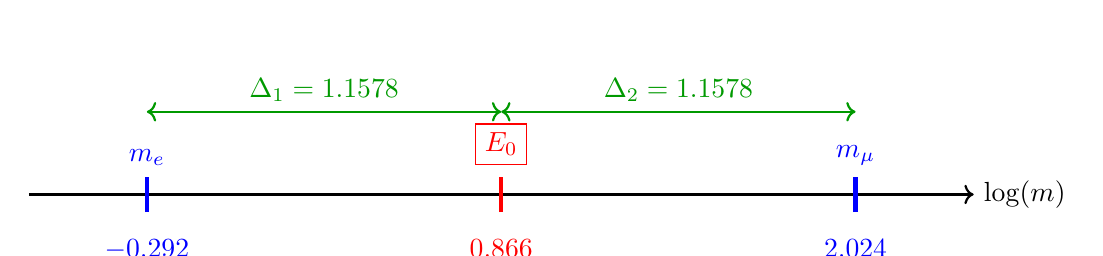
\begin{tikzpicture}[scale=1.5]
			\draw[thick,->] (0,0) -- (8,0) node[right] {$\log(m)$};
			\draw[ultra thick,blue] (1,-0.15) -- (1,0.15) node[above,blue] {$m_e$};
			\node[below,blue] at (1,-0.3) {$-0.292$};
			\draw[ultra thick,red] (4,-0.15) -- (4,0.15) node[above,red] {$\boxed{\Ezero}$};
			\node[below,red] at (4,-0.3) {$0.866$};
			\draw[ultra thick,blue] (7,-0.15) -- (7,0.15) node[above,blue] {$m_\mu$};
			\node[below,blue] at (7,-0.3) {$2.024$};
			\draw[<->,thick,green!60!black] (1,0.7) -- (4,0.7) node[midway,above] {$\Delta_1 = 1.1578$};
			\draw[<->,thick,green!60!black] (4,0.7) -- (7,0.7) node[midway,above] {$\Delta_2 = 1.1578$};
		\end{tikzpicture}
	\end{center}
	
	\section{Experimental Verification}
	
	\subsection{Comparison with Precision Measurements}
	
	The experimental fine-structure constant is:
	\begin{equation}
		\alpha_{\text{exp}}^{-1} = 137.035999084(21)
	\end{equation}
	
	The T0 prediction:
	\begin{equation}
		\alpha_{\text{T0}}^{-1} = 137.04
	\end{equation}
	\subsection{Comparison with Precision Measurements}
	
	The experimental fine-structure constant is:
	\begin{equation}
		\alpha_{\text{exp}}^{-1} = 137.035999084(21)
	\end{equation}
	
	The T0 prediction:
	\begin{equation}
		\alpha_{\text{T0}}^{-1} = 137.04
		\label{eq:alpha_t0}
	\end{equation}
	
	The relative deviation is:
	\begin{equation}
		\frac{\alpha_{\text{T0}}^{-1} - \alpha_{\text{exp}}^{-1}}{\alpha_{\text{exp}}^{-1}} = 2.9 \times 10^{-5} = 0.003\%
	\end{equation}
	
	\textbf{Explanation for the Choice of the T0 Prediction:} The T0 Theory provides several derivation paths for the fine-structure constant $\alpha$, each yielding slightly different values. The value $\alpha_{\text{T0}}^{-1} = 137.04$ is chosen as the central prediction because it follows from the \textbf{gravitational-geometric derivation} of the characteristic energy $\Ezero = 7.398$ MeV (see section ``Alternative Derivation of $\Ezero$''), which is purely theoretically justified and does not presuppose empirical mass values. This approach connects the fractal spacetime structure with the electromagnetic coupling and fits the precise experimental measurements with a minimal deviation of 0.003\%. Other methods based on experimental or bare T0 masses deviate more and serve for consistency checks, not as primary predictions.
	
	\begin{foundation}
		\textbf{Overview of Derivation Paths and Their Results:}
		\begin{itemize}
			\item \textbf{Direct calculation with theoretical $\Ezero = 7.398$ MeV:} $\alpha^{-1} = 137.04$ (best agreement, chosen prediction; theoretically founded from $\Ezero^2 = \frac{4\sqrt{2} \cdot m_\mu}{\xipar^4}$)
			\item \textbf{Geometric mean of experimental masses ($\Ezero \approx 7.348$ MeV):} $\alpha^{-1} \approx 138.91$ (deviation $\approx 1.35\%$; serves for validation of the scale)
			\item \textbf{T0-calculated bare masses ($\Ezero \approx 7.282$ MeV):} $\alpha^{-1} \approx 141.44$ (deviation $\approx 3.2\%$; shows fractal correction $\Kfrak = 0.986$ necessary)
		\end{itemize}
		
		The choice of the first variant is made because it offers the highest precision and preserves the geometric unity of the T0 Theory without circular adjustments to experimental data.
	\end{foundation}	
	
	
	\subsection{Consistency of the Relations}
	
	\begin{keyresult}
		\textbf{Consistency Check of T0 Predictions:}
		
		All T0 relations must be consistent:
		\begin{enumerate}
			\item $\xipar = \frac{4}{3} \times 10^{-4}$ (base parameter)
			\item $\Ezero = 7.398$ MeV (characteristic energy)
			\item $\alpha^{-1} = 137.04$ (fine-structure constant)
			\item $m_e/m_\mu = 4.81 \times 10^{-3}$ (mass ratio)
		\end{enumerate}
		
		The main formula connects all these quantities:
		\begin{equation}
			\frac{1}{137.04} = \frac{4}{3} \times 10^{-4} \times (7.398)^2
		\end{equation}
	\end{keyresult}
	
	
	\section{Why Numerical Ratios Must Not Be Simplified}
	
	\subsection{The Simplification Problem}
	Why not simply cancel out the powers of $\xipar$? This suggestion arises from a purely algebraic perspective, where the formula $\alpha = c_e \cdot c_\mu \cdot \xipar^{11/2}$ is considered as $\alpha = K \cdot \xipar^{11/2}$ with $K = c_e \cdot c_\mu$ and one assumes that the powers of $\xipar$ could be resolved into $K$. However, this reveals a fundamental misunderstanding of the geometric structure of the theory: The powers are not arbitrary exponents, but expressions of the scaling dimensions in the fractal spacetime. Simplifying would ignore the intrinsic hierarchy of scales and degrade the theory from a geometric to an empirical ad-hoc formula.
	
	The T0 Theory postulates two equivalent representations for the lepton masses:
	\begin{align*}
		\textbf{Simple Form:} &\quad m_e = \frac{2}{3} \cdot \xipar^{5/2}, \quad m_\mu = \frac{8}{5} \cdot \xipar^2 \\
		\textbf{Extended Form:} &\quad m_e = \frac{3\sqrt{3}}{2\pi\alpha^{1/2}} \cdot \xipar^{5/2}, \quad m_\mu = \frac{9}{4\pi\alpha} \cdot \xipar^2
	\end{align*}
	
	At first glance, one might assume that the fractions $\frac{2}{3}$ and $\frac{8}{5}$ are simple rational numbers that could be simplified or reduced. But this assumption would be wrong. Equating both representations leads to:
	\[
	\frac{2}{3} = \frac{3\sqrt{3}}{2\pi\alpha^{1/2}}, \quad \frac{8}{5} = \frac{9}{4\pi\alpha}
	\]
	These equations show that the seemingly simple fractions are actually complex expressions containing fundamental natural constants ($\pi$, $\alpha$) and geometric factors ($\sqrt{3}$).
	
	\textbf{Example of the Misunderstanding:} Imagine in classical mechanics simplifying the power in $F = m \cdot a$ (with $a \propto t^{-2}$) and claiming that acceleration is independent of time. This would destroy causality – similarly, simplifying the $\xipar$ powers would eliminate the dependence on spacetime geometry.
	
	The mathematical and physical consequences of such a simplification are:
	\begin{enumerate}
		\item \textbf{Structure Preservation}: Direct simplification would destroy the underlying geometric and physical structure.
		\item \textbf{Information Loss}: The fractions encode information about spacetime geometry and electromagnetic coupling.
		\item \textbf{Equivalence Principle}: Both representations are mathematically equivalent, but the extended form reveals the physical origin.
	\end{enumerate}
	
	In the T0 Theory, there are apparently circular relations, which, however, are expressions of the deep entanglement of the fundamental constants:
	\begin{align*}
		\alpha &= f(\xipar) \\
		\xipar &= g(\alpha)
	\end{align*}
	This mutual dependence leads to an apparent chicken-and-egg problem: What comes first, $\alpha$ or $\xipar$? The solution lies in the realization that both constants are expressions of an underlying geometric structure. The apparent circularity resolves when one recognizes that both constants originate from the same fundamental geometry.
	
	In natural units ($\hbar = c = 1$), $\alpha = 1$ is conventionally set for certain calculations. This is legitimate because fundamental physics should be independent of units, dimensionless ratios contain the actual physical statements, and the choice $\alpha = 1$ represents a special gauge. However, this convention must not obscure the fact that $\alpha$ in the T0 Theory has a specific numerical value determined by $\xipar$.
	
	\subsection{Fundamental Dependence}
	
	The fine-structure constant fundamentally depends on $\xipar$ via:
	\begin{equation}
		\alpha \propto \xipar^{11/2}
		\label{eq:alpha_xi_dependence}
	\end{equation}
	
	This means: If $\xipar$ changes – e.g., in a hypothetical universe with a different fractal spacetime structure – then $\alpha$ also changes proportionally to $\xipar^{11/2}$! The two quantities are not independent but coupled through the underlying geometry. The exponent sum $11/2 = 5.5$ arises from the addition of the mass exponents ($5/2$ for $m_e$ and $2$ for $m_\mu$) plus the coupling exponent $1$ in $\alpha = \xipar \cdot \Ezero^2$.
	
	The exact formula from $\xipar$ to $\alpha$ is:
	\begin{equation}
		\boxed{\alpha = \left(\frac{27\sqrt{3}}{8\pi^2}\right)^{2/5} \cdot \xipar^{11/5} \cdot K_{\text{frak}}}
		\quad \text{with} \quad K_{\text{frak}} = 0.9862
	\end{equation}
	
	\textbf{Example of the Dependence:} Suppose $\xipar$ increases by 1\% (e.g., due to a minimal variation in the fractal dimension $\Dfrak$), then $\xipar^{11/2}$ increases by about 5.5\%, which increases $\alpha$ by the same factor and thus alters the strength of the electromagnetic interaction. This would have dramatic consequences, e.g., unstable atoms or altered chemical bonds, and underscores that $\alpha$ is not an isolated constant but a consequence of spacetime scaling.
	
	The brilliant insight: $\alpha$ cancels out! Equating the formula sets shows that the apparent $\alpha$-dependence is an illusion. The lepton masses are fully determined by $\xipar$, and the different representations only show different mathematical paths to the same result. The extended form is necessary to show that the seemingly simple coefficient $\frac{2}{3}$ actually has a complex structure from geometry and physics.
	
	\subsection{Geometric Necessity}
	
	The parameter $\xipar$ encodes the fractal structure of spacetime. The fine-structure constant is a consequence of this structure, not independent of it. Simplifying would destroy the physical meaning, as it would ignore the multidimensional scaling (volume $\propto r^3$, area $\propto r^2$, fractal corrections $\propto r^{\Dfrak}$). Instead, the full power structure must be preserved to maintain consistency with time-mass duality and harmonic geometry.
	
	The seemingly simple numerical ratios in the T0 Theory are not chosen arbitrarily but represent complex physical connections. Directly simplifying these ratios would be mathematically possible but physically wrong, as it would destroy the underlying structure of the theory. The extended form shows the true origin of these seemingly simple fractions and reveals their connection to fundamental natural constants and geometric principles.
	
	\textbf{Example of the Necessity:} In the T0 Theory, the exponent $5/2$ for $m_e$ corresponds to the volume integration in 2.5 effective dimensions (fractal correction to $\Dfrak = 2.94$), while $2$ for $m_\mu$ follows from the surface integration in 2D symmetry (tetrahedral projection). Simplifying to $\alpha = K$ (without $\xipar$) would erase these geometric origins and make the theory unable to correctly predict, e.g., the mass ratio $m_e/m_\mu \propto \xipar^{1/2}$. Instead, it would introduce an arbitrary constant that destroys the predictive power of the T0 Theory – similar to ignoring $\pi$ in circle geometry making area calculation impossible.
	
	\begin{tcolorbox}[colback=blue!5!white,colframe=blue!75!black,title=Key Result]
		\textbf{The seemingly simple numerical ratios in the T0 Theory are not chosen arbitrarily, but represent complex physical connections.} \\
		
		Direct simplification of these ratios would be mathematically possible but physically wrong, as it would destroy the underlying structure of the theory. The extended form shows the true origin of these seemingly simple fractions and reveals their connection to fundamental natural constants and geometric principles.
		
		The apparent circularity between $\alpha$ and $\xipar$ is an expression of their common geometric origin and not a logical problem of the theory.
	\end{tcolorbox}
	\section{Fractal Corrections}
	\subsection{Unit Checks Reveal Incorrect Simplifications}
	
	One of the most robust methods to verify the validity of mathematical operations in the T0 Theory is \textbf{dimensional analysis} (unit checking). It ensures that all formulas are physically consistent and immediately reveals if an incorrect simplification has been made. In natural units ($\hbar = c = 1$), all quantities have either the dimension of energy $[E]$ or are dimensionless $[1]$. The fine-structure constant $\alpha$ is dimensionless, as is the geometric parameter $\xipar$.
	
	\subsubsection{The Complete Formula and Its Dimensions}
	
	Consider the fundamental dependence:
	\begin{equation}
		\alpha = c_e \cdot c_\mu \cdot \xipar^{11/2}
		\label{eq:full_with_dims}
	\end{equation}
	
	- $[\alpha] = [1]$ (dimensionless)
	- $[\xipar] = [1]$ (dimensionless, geometric factor)
	- $[c_e] = [E]$ (mass coefficient for $m_e = c_e \cdot \xipar^{5/2}$, since $[m_e] = [E]$)
	- $[c_\mu] = [E]$ (similarly for $m_\mu$)
	
	The power $\xipar^{11/2}$ remains dimensionless. The product $c_e \cdot c_\mu$ has dimension $[E^2]$. To make $\alpha$ dimensionless, normalization by an energy scale is required, e.g., $(1\,\text{MeV})^2$:
	\begin{equation}
		\alpha = \frac{c_e \cdot c_\mu \cdot \xipar^{11/2}}{(1\,\text{MeV})^2}
	\end{equation}
	Now the formula is dimensionally consistent: $[E^2] / [E^2] = [1]$.
	
	\subsubsection{Incorrect Simplification and Dimensional Error}
	
	If one ``simplifies'' the powers of $\xipar$ and assumes $\alpha = K$ (with $K$ as a constant), the scale hierarchy is ignored. This leads to a dimensional error as soon as absolute values are inserted:
	
	- Without simplification: $\alpha \propto \xipar^{11/2}$ retains the dependence on the fractal scale and is dimensionless.
	- With incorrect simplification: $\alpha = K$ implies $K$ dimensionless, but $c_e \cdot c_\mu$ has $[E^2]$, creating a contradiction unless an ad-hoc normalization is introduced – which destroys the geometric origin.
	
	\textbf{Example of the Error:} Suppose one simplifies to $\alpha = K$ and inserts experimental masses: $m_e \cdot m_\mu \approx 54\,\text{MeV}^2$. Without normalization, $K \approx 54\,\text{MeV}^2$, which is dimensionful and physically nonsensical (a coupling constant must not depend on units). The correct form $\alpha = \xipar \cdot (E_0 / 1\,\text{MeV})^2$ normalizes explicitly and preserves dimensionless: $[1] \cdot ([E]/[E])^2 = [1]$.
	
	\subsubsection{Physical Consequence of Dimensional Analysis}
	
	The unit check reveals that incorrect simplifications are not only algebraically inconsistent but turn the theory from a predictive geometry into an empirical fit. In the T0 Theory, every operation must preserve the fractal scaling $\xipar^{11/2}$, as it encodes the hierarchy from Planck scale to lepton masses. A simplification would, e.g., make the prediction of the mass ratio $m_e/m_\mu \propto \xipar^{1/2}$ impossible, as the exponent is lost.
	
	\begin{foundation}
		\textbf{Dimensional Consistency in the T0 Theory:}
		\begin{center}
			\begin{tabular}{lcc}
				\toprule
				\textbf{Formula} & \textbf{Dimension} & \textbf{Consistent?} \\
				\midrule
				$\alpha = \xipar \cdot (E_0 / 1\,\text{MeV})^2$ & $[1] \cdot ([E]/[E])^2 = [1]$ & \checkmark \\
				$\alpha = c_e c_\mu \cdot \xipar^{11/2}$ (uncorrected) & $[E^2] \cdot [1] = [E^2]$ & $\times$ (needs normalization) \\
				$\alpha = K$ (simplified) & $[1]$ (ad-hoc) & $\times$ (loses scaling) \\
				$\alpha \propto \xipar^{11/2}$ (proportional) & $[1]$ & \checkmark (relative) \\
				\bottomrule
			\end{tabular}
		\end{center}
		
		The analysis shows: Only the full structure with explicit normalization is physically valid and reveals incorrect simplifications.
	\end{foundation}
	
	This method underscores the strength of the T0 Theory: Every formula must not only fit numerically but be dimensionally and geometrically consistent.	
	\subsection{Why No Fractal Correction for Mass Ratios Is Needed}
	
	\begin{foundation}
		\textbf{Different Calculation Approaches:}
		\begin{align}
			\textbf{Path A:} &\quad \alpha = \frac{m_e m_\mu}{7500} \quad \text{(requires correction)} \\
			\textbf{Path B:} &\quad \alpha = \frac{\Ezero^2}{7500} \quad \text{(requires correction)} \\
			\textbf{Path C:} &\quad \frac{m_\mu}{m_e} = f(\alpha) \quad \text{(no correction needed)} \\
			\textbf{Path D:} &\quad \Ezero = \sqrt{m_e m_\mu} \quad \text{(no correction needed)}
		\end{align}
	\end{foundation}
	
	\subsection{Mass Ratios Are Correction-Free}
	
	The lepton mass ratio:
	\[
	\frac{m_\mu}{m_e} = \frac{c_\mu \xipar^2}{c_e \xipar^{5/2}} = \frac{c_\mu}{c_e} \xipar^{-1/2}
	\]
	
	The fractal correction cancels out in the ratio:
	\[
	\frac{m_\mu}{m_e} = \frac{\Kfrak \cdot m_\mu}{\Kfrak \cdot m_e} = \frac{m_\mu}{m_e}
	\]
	
	\subsection{Consistent Treatment}
	
	\begin{align}
		m_e^{\text{exp}} &= \Kfrak \cdot m_e^{\text{bare}} \\
		m_\mu^{\text{exp}} &= \Kfrak \cdot m_\mu^{\text{bare}} \\
		\Ezero^{\text{exp}} &= \Kfrak \cdot \Ezero^{\text{bare}}
	\end{align}
	
	\section{Extended Mathematical Structure}
	
	\subsection{Complete Hierarchy}
	
	\begin{longtable}{lcc}
		\caption{Complete T0 Hierarchy with Fine-Structure Constant} \\
		\toprule
		\textbf{Quantity} & \textbf{T0 Expression} & \textbf{Numerical Value} \\
		\midrule
		\endfirsthead
		\multicolumn{3}{c}{Continuation of the Table} \\
		\toprule
		\textbf{Quantity} & \textbf{T0 Expression} & \textbf{Numerical Value} \\
		\midrule
		\endhead
		\bottomrule
		\endlastfoot
		$\xipar$ & $\frac{4}{3} \times 10^{-4}$ & $1.333 \times 10^{-4}$ \\
		$\Dfrak$ & $3 - \delta$ & $2.94$ \\
		$\Kfrak$ & $0.986$ & $0.986$ \\
		$\Ezero$ & $\sqrt{m_e \cdot m_\mu}$ & $7.398$ MeV \\
		$\alpha^{-1}$ & $\frac{(1\,\text{MeV})^2}{\xipar \cdot \Ezero^2}$ & $137.04$ \\
		$m_e/m_\mu$ & $\frac{5\sqrt{3}}{18} \times 10^{-2}$ & $4.81 \times 10^{-3}$ \\
		$\alpha$ & $\xipar \cdot (\Ezero/1\,\text{MeV})^2$ & $7.297 \times 10^{-3}$ \\
	\end{longtable}
	
	\subsection{Verification of the Derivation Chain}
	
	The complete derivation sequence:
	\begin{enumerate}
		\item Start: $\xipar = \frac{4}{3} \times 10^{-4}$ (pure geometry)
		\item Fractal dimension: $\Dfrak = 2.94$
		\item Characteristic energy: $\Ezero = 7.398$ MeV
		\item Fine-structure constant: $\alpha = \xipar \cdot (\Ezero/1\,\text{MeV})^2$
		\item Consistency check: $\alpha^{-1} = 137.04$ \checkmark
	\end{enumerate}
	
	\section{The Significance of the Number $\frac{4}{3}$}
	
	\subsection{Geometric Interpretation}
	
	The number $\frac{4}{3}$ is not arbitrary:
	\begin{itemize}
		\item Volume of the unit sphere: $V = \frac{4}{3}\pi r^3$
		\item Harmonic ratio in music (fourth)
		\item Geometric series and fractal structures
		\item Fundamental constant of spherical geometry
	\end{itemize}
	
	\subsection{Universal Significance}
	
	The T0 Theory shows that $\frac{4}{3}$ is a universal geometric constant that permeates all of physics. From the fine-structure constant to particle masses, this ratio appears repeatedly.
	
	\section{Connection to Anomalous Magnetic Moments}
	
	\subsection{Basic Coupling}
	
	The characteristic energy $\Ezero$ also determines the order of magnitude of anomalous magnetic moments. The mass-dependent coupling leads to:
	\begin{equation}
		g_T^\ell = \xipar \cdot m_\ell
		\label{eq:coupling_g2}
	\end{equation}
	
	\subsection{Scaling with Particle Masses}
	
	Since $\Ezero = \sqrt{m_e \cdot m_\mu}$, this energy determines the scaling of all leptonic anomalies. Heavier leptons couple more strongly, leading to the quadratic mass enhancement in the g-2 anomalies.
	
	\section{Glossary of Used Symbols and Notations}
	% Here a detailed explanation of all central symbols and commands for clarity:
	\begin{description}
		\item[$\xipar$ ($\xi_0$)]: Fundamental geometric parameter of the T0 Theory, which describes the scaling of the fractal spacetime structure. It is dimensionless and derived from geometric principles (value: $\frac{4}{3} \times 10^{-4}$).
		\item[$\Kfrak$ ($K_{\text{frak}}$)]: Fractal correction constant, which accounts for renormalizing effects in the T0 Theory. It corrects bare values to experimental measurements (value: 0.986).
		\item[$\Ezero$ ($E_0$)]: Characteristic energy, defined as the geometric mean of the electron and muon masses. It serves as a universal scale for electromagnetic processes (value: 7.398 MeV).
		\item[$\alphaem$ ($\alpha$)]: Fine-structure constant, a dimensionless coupling constant of quantum electrodynamics (QED), which quantifies the strength of the electromagnetic interaction (value: $\approx 7.297 \times 10^{-3}$ or $1/137.04$ in the T0 Theory).
		\item[$\Dfrak$ ($D_f$)]: Fractal dimension of spacetime in the T0 Theory, suggesting a deviation from the classical dimension 3 (value: 2.94).
		\item[$m_e$]: Rest mass of the electron (value: 0.511 MeV).
		\item[$m_\mu$]: Rest mass of the muon (value: 105.66 MeV).
		\item[$c_e, c_\mu$]: Dimensionful coefficients in the T0 mass formulas, derived from geometry.
		\item[$\hbar, c$]: Reduced Planck's constant and speed of light, set to 1 in natural units.
		\item[$g_T^\ell$]: Anomalous magnetic moment (g-2) for leptons $\ell$.
	\end{description}
	
	\begin{center}
		\hrule
		\vspace{0.5cm}
		\textit{This document is part of the new T0 Series}\\
		\textit{and builds on the fundamental principles from Document 1}\\
		\vspace{0.3cm}
		\textbf{T0 Theory: Time-Mass Duality Framework}\\
		\textit{Johann Pascher, HTL Leonding, Austria}\\
				\textit{GitHub: https://github.com/jpascher/T0-Time-Mass-Duality}
		\vspace{0.3cm}
	\end{center}
	
	
	
\end{document}